\section{State-Of-The-Art Analyse}

\subsection{Betrachtungsgegenstand}
Der derzeitige State-Of-The-Art im Bereich \ac{T2P} ist das Verfahren von Friedrich aus dem Jahr 2011 (\cite[vgl.][11]{RIEFER}). Im Folgenden wird die von Friedrich erarbeitete Vorgehensweise (\cite[vgl.][]{FRIEDRICH1} und \cite[vgl.][]{FRIEDRICH2}) analysiert und Verbesserungsvorschläge erarbeitet. Die Analyse beschränkt sich auf die Textverarbeitung und die daraus resultierende Generierung des World Models. Die Konstruktion eines Graphen aus dem World Model ist nicht Teil dieser Arbeit.
\par
Zunächst wird im Folgenden kurz auf den konkreten Aufbau des World Models nach Friedrich eingegangen. Anschließend folgt die Analyse der Vorgehensweise. Gemäß der durch Friedrich vorgegebenen Gliederung wird zunächst die Textverarbeitung auf Satz-Ebene und dann die Textverarbeitung auf Text-Ebene analysiert. Abschließend werden bekannte Problemfelder zusammengetragen und Lösungsansätze vorgeschlagen.

\subsection{World Model}
Die Verwendung einer World-Model-Datenstruktur als Zwischenspeicher für die aus einem Text extrahierten Informationen ist üblich. Friedrich greift auf bestehende Ansätze zurück und modifiziert die Datenstruktur, sodass später ein \ac{BPMN}-Graph abgeleitet werden kann.
\par
Das World Model nach Friedrich beinhaltet 8 Klassen (\cite[vgl.][46]{FRIEDRICH2}). 

\begin{itemize} 
\item ORIGINATED ELEMENT: Aus einem Text extrahierte Entität. Um Rückverfolgbarkeit zu ermöglichen wird hier eine Referenz zum Ursprungssatz hinterlegt.
\item SPECIFIED ELEMENT: Verfeinerung des \textit{Originated Element}. Speicher einen Bezug zu einem Wort im Text und wird genutzt um mit \textit{Specifiern} zu interagieren.
\item SPECIFIER: Annotierte Information, die zur genaueren Spezifikation eines \textit{Specified Element} dient.
\item EXTRACTED OBJECT: Textpart, der vom Hauptsatz extrahiert wurde. Es erbt vom \textit{Specified Element} und wird  von \textit{Actor} und \textit{Resource} genauer spezifiziert.
\item ACTOR: Subjekt eines Satzes, das als agierende Entität zu verstehen ist. 
\item RESOURCE: Objekt eines Satzes.
\item ACTION: Aus dem Text extrahierte Aktivität, die einen \textit{Actor} und eine \textit{Resource} besitzen kann. Eine Aktivität kann mit weiteren Aktivitäten verbunden werden.
\item FLOW: Repräsentiert die Beziehungen zwischen Aktivitäten. Es wird zwischen den beiden Möglichkeiten \textit{Split-Flow} und \textit{Join-Flow} unterschieden. Darüber hinaus spezifiziert der Typ, ob es sich um gleichzeitige, sequenziell ablaufende, Entscheidungs- oder Ausnahme-Relationen handelt.
\end{itemize}

Der korrekte Aufbau dieses World Models aus dem Text ist Grundvoraussetzung für die erfolgreiche Erstellung eines Graphen. Es entsteht Schritt für Schritt durch die Folgenden Verarbeitungsschritte.

\subsection{Textverarbeitung auf Satz-Ebene}

Der Eingangstext in natürlicher Sprache wird zunächst in einzelne Wörter und Sätze aufgesplittet. In \ref{fig:SLEVEL} wird dieser Vorgang der \textit{Sentence Decomposition} zugeordnet. Es handelt sich hierbei um eine normale Tokenization, bei der auf die Stanford CoreNLP Funktionen \textit{Stanford TokenizerAnnotator} und \textit{Stanford WordsToSentenceAnnotator} zurückgegriffen wird. Im nächsten Schritt wird der Text mit dem \textit{POSTaggerAnnotator} mit \textit{POS-Tags} versehen und anschließend mit dem PCFG-Parser \textit{ParserAnnotator} die Satzstruktur analysiert. Dies wird durch den Pfeil von StanfordParser zu Subprozess in \ref{fig:SLEVEL} symbolisiert. Auf eine pauschale \textit{Lemmatization} aller Wörter wird an dieser Stelle verzichtet. Die zwei weiteren an dieser Stelle üblichen Standard-Analysemöglichkeiten \textit{Collocation Extraction} (Erkennen von zusammengesetzten Wörtern) und \textit{Named Entity Recognition} (Analyse von Eigennamen) werden ebenfalls nicht genutzt.
\par
\begin{wrapfigure}{r}{13cm}
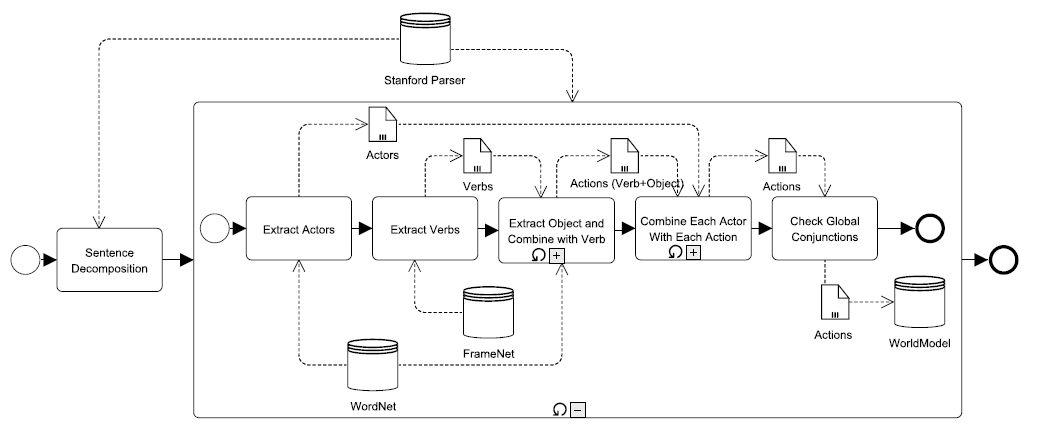
\includegraphics[width=13cm]{pictures/SentenceLevel.png}
\caption{Analyseschema auf Satzebene (\cite[vgl.][5]{FRIEDRICH2})}
\label{fig:SLEVEL}
\end{wrapfigure}
\par

Auf Basis der Annotationen folgt dann das \textit{Phrase Chunking}, der zweite Teil der Sentence Decomposition. Hierzu analysiert ein von Friedrich selbst entwickelter Algorithmus die Informationen zur Satzstruktur (\cite[vgl.][49]{FRIEDRICH2}). Haupt-und Nebensätze werden identifiziert und  auf Abhängigkeiten untersucht. Nebensätze werden als irrelevant klassifiziert und herausgefiltert, wenn keine Abhängigkeit zum Hauptsatz besteht. Relativsätze werden zunächst ignoriert.
\par
Der in \ref{fig:SLEVEL} dargestellte Subprozess wird von Friedrich als \textit{Element Extraction} bezeichnet und umfasst die semantische Analyse auf Satz-Ebene. Zunächst wird der Actor aus dem Satz extrahiert. Bei einem Satz im Aktiv, wird hierfür nach einem Specified Object mit dem Specifier \textit{nsubj} \footnote{Eine kurze Erläuterung der Stanford-Dependency-Kürzel findet sich hier: //nlp-ml.io/jg/software/pac/standep.html} gesucht. Bei einem Satz im passiv nach einem Specified Object mit Specifier \textit{agent}. Wird ein Actor gefunden, kann ein Actor-Objekt erstellt, mit Zusatzinformationen über mögliche logische Konjunktionen versehen und in einer Liste gespeichert werden. Als nächstes wird die Action identifiziert.  Eine Action ist im Gegensatz zu einem Actor nicht optional. Eine Action basiert immer auf einem Verb. Dieses findet sich entweder über die \textit{nsubj}-, die \textit{cop}- oder die \textit{dobj}-Beziehung. Bei Sätzen im Passiv ist die \textit{nsubjpass}-Relation Aufschluss gebend. Auf vergleichbare Art werden die zum Verb gehörenden Objekte extrahiert und mit Hilfe von WordNet als Actor oder Resource klassifiziert. Anschließend werden zum Verb gehörende Relativsätze analysiert und dann alles mit Zusatznformationen über mögliche logische Konjunktionen und in einer zweiten Liste gespeichert. Die Identifikation und Handhabung von logischen Konjunktionen \footnote{Logische AND-Verknüpfungen wie beispielsweise in: \textit{He reads AND drinks coffee.}} erfolgt ebenfalls mittels eines eigenen Algorithmus. Im letzten Schritt des Subprozesses erfolgt die Speicherung der Informationen im Worldmodel.
\par
Die Identifikation der semantischen Rollen erfolgt hier folglich komplett regelbasiert über die Syntax-Annotationen mittels eines von Friedrich entwickelten Algorithmus. Zwar wird FrameNet eingesetzt, um Objekten auf Basis ihres Beszugsverbes ein Frame Element zuzuordnen, doch auf ein bestehendes \ac{SRL}-Tool wird nicht zurückgegriffen. Die Klassifikation eines Objektes als Actor oder Resource mittels WordNet könnte durch Named Entity Recognition und einen Word-Sense-Disambiguation-Algorithmus verbessert werden.

\subsection{Textverarbeitung auf Text-Ebene}
\begin{figure}[H]
\begin{center}

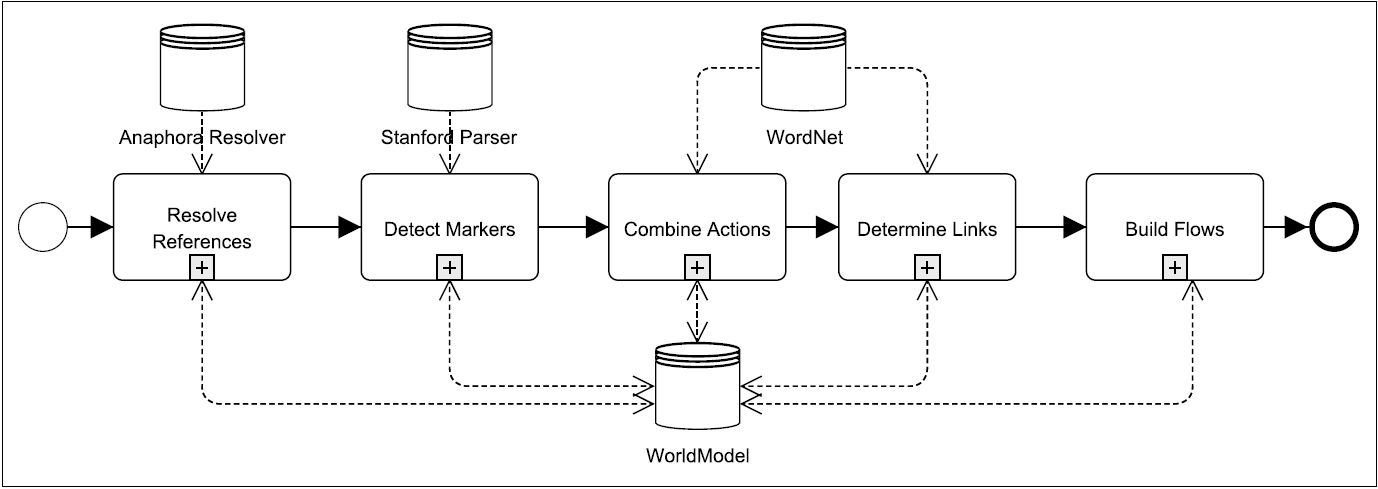
\includegraphics[keepaspectratio=true, width=\textwidth]{pictures/textLevel.png}
\caption{Analyseschema auf Textebene}
\label{fig:TLEVEL}
\end{center}\end{figure}

Anaphora Resolution: Wichtig für Beziehungen zwischen Sätzen, Stanford kann coref

Detect Markers:  

Combine Actions:

Determine Links:

Build Flows:

\subsection{Problemfelder und Lösungsansätze}
Kann vielleicht auch in den Ausblick.



